\section{Design of the Delay and \gls{reverb} Effect}
In this section, the delay and the \gls{reverb} will be designed to fit intro a \gls{dsp}, which mean that a discreet block diagram is obtained and afterwords the equation to the implementation is made. All the equation will afterwords be simulated in MATLAB and then the assembly code is developed and implemented. 


\subsection{Obtaining the Differential Equation}
The Delay and \gls{reverb} effect are very similar in their design so they will be presented and designed in the same section. The block diagram presented in \autoref{} is changed so it fit intro a direct form 2 construction. This effect both have \gls{iir} filter and \gls{fir} filter, but it is only the \gls{iir} filter which make the echo, the \gls{fir} filter is only applied to make a flat frequency respond. To get a naturally \gls{reverb} effect with the identical respond as a room acustic respond and avoiding fluttering, all the seriel \gls{reverb} unit needs to be an all pass filter and all parallel \gls{reverb} unit needs to be low pass filter. The low pass filter is used because the room akustic caristica is acting as a low pass filter, all low frequency signal will stay longer in the room than the high frequency \autoref{}.  The \gls{reverb} needs to have at least 1000 echo per second, and the best way to make the \gls{reverb} effect is with four low pass \gls{iir} filters and 2 all pass filter otherwise if all the all pass filter was in parallel, it will require forty all pass filter to make 1000 echo per second \citep{natural_sounding_revorb}. The block diagram \autoref{fig:reverb_block_des} is in direct form 2 to minimize the implementation program. The delay and \gls{reverb} effect can be obtained and is shown in \autoref{fig:reverb_block_des}. The \gls{reverb} effect is the one in red and black while the delay is only in red. 

\newpage

\begin{figure} [htbp]
 \centering
\begin{picture}(0,0)%
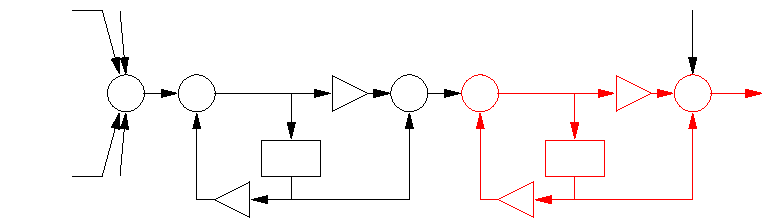
\includegraphics{reverb_diag_des.pdf}%
\end{picture}%
\setlength{\unitlength}{4144sp}%
%
\begingroup\makeatletter\ifx\SetFigFont\undefined%
\gdef\SetFigFont#1#2#3#4#5{%
  \reset@font\fontsize{#1}{#2pt}%
  \fontfamily{#3}\fontseries{#4}\fontshape{#5}%
  \selectfont}%
\fi\endgroup%
\begin{picture}(5832,1599)(-1319,-1288)
\put(2656,-106){\makebox(0,0)[lb]{\smash{{\SetFigFont{12}{14.4}{\rmdefault}{\mddefault}{\updefault}{\color[rgb]{1,0,0}$w_6[n]$}%
}}}}
\put(1711,-421){\makebox(0,0)[lb]{\smash{{\SetFigFont{12}{14.4}{\rmdefault}{\mddefault}{\updefault}{\color[rgb]{0,0,0}$\Sigma$}%
}}}}
\put(721,-916){\makebox(0,0)[lb]{\smash{{\SetFigFont{12}{14.4}{\rmdefault}{\mddefault}{\updefault}{\color[rgb]{0,0,0}$z^{-d_5}$}%
}}}}
\put( 91,-421){\makebox(0,0)[lb]{\smash{{\SetFigFont{12}{14.4}{\rmdefault}{\mddefault}{\updefault}{\color[rgb]{0,0,0}$\Sigma$}%
}}}}
\put(1261,-196){\makebox(0,0)[lb]{\smash{{\SetFigFont{12}{14.4}{\rmdefault}{\mddefault}{\updefault}{\color[rgb]{0,0,0}$-a_5$}%
}}}}
\put(2251,-421){\makebox(0,0)[lb]{\smash{{\SetFigFont{12}{14.4}{\rmdefault}{\mddefault}{\updefault}{\color[rgb]{1,0,0}$\Sigma$}%
}}}}
\put(2881,-916){\makebox(0,0)[lb]{\smash{{\SetFigFont{12}{14.4}{\rmdefault}{\mddefault}{\updefault}{\color[rgb]{1,0,0}$z^{-d_6}$}%
}}}}
\put(271,-1006){\makebox(0,0)[lb]{\smash{{\SetFigFont{12}{14.4}{\rmdefault}{\mddefault}{\updefault}{\color[rgb]{0,0,0}$a_5$}%
}}}}
\put(2431,-1006){\makebox(0,0)[lb]{\smash{{\SetFigFont{12}{14.4}{\rmdefault}{\mddefault}{\updefault}{\color[rgb]{1,0,0}$a_6$}%
}}}}
\put(3871,-421){\makebox(0,0)[lb]{\smash{{\SetFigFont{12}{14.4}{\rmdefault}{\mddefault}{\updefault}{\color[rgb]{1,0,0}$\Sigma$}%
}}}}
\put(3421,-196){\makebox(0,0)[lb]{\smash{{\SetFigFont{12}{14.4}{\rmdefault}{\mddefault}{\updefault}{\color[rgb]{1,0,0}$-a_6$}%
}}}}
\put(-449,-421){\makebox(0,0)[lb]{\smash{{\SetFigFont{12}{14.4}{\rmdefault}{\mddefault}{\updefault}{\color[rgb]{0,0,0}$\Sigma$}%
}}}}
\put(-224,-106){\makebox(0,0)[lb]{\smash{{\SetFigFont{12}{14.4}{\rmdefault}{\mddefault}{\updefault}{\color[rgb]{0,0,0}$x_5[n]$}%
}}}}
\put(1936,-106){\makebox(0,0)[lb]{\smash{{\SetFigFont{12}{14.4}{\rmdefault}{\mddefault}{\updefault}{\color[rgb]{1,0,0}$x_6[n]$}%
}}}}
\put(4276,-106){\makebox(0,0)[lb]{\smash{{\SetFigFont{12}{14.4}{\rmdefault}{\mddefault}{\updefault}{\color[rgb]{1,0,0}$y[n]$}%
}}}}
\put(-1304,-151){\makebox(0,0)[lb]{\smash{{\SetFigFont{12}{14.4}{\rmdefault}{\mddefault}{\updefault}{\color[rgb]{0,0,0}Low pass}%
}}}}
\put(-1304,-421){\makebox(0,0)[lb]{\smash{{\SetFigFont{12}{14.4}{\rmdefault}{\mddefault}{\updefault}{\color[rgb]{0,0,0}filter in}%
}}}}
\put(-1304,-646){\makebox(0,0)[lb]{\smash{{\SetFigFont{12}{14.4}{\rmdefault}{\mddefault}{\updefault}{\color[rgb]{0,0,0}Parallel}%
}}}}
\end{picture}%

  \caption{The figure shows a block diagram of a \gls{reverb} and delay unit.}
  \label{fig:reverb_block_des}
\end{figure}

From \autoref{fig:reverb_block_des}, the following differential equations can be inferred for the delay, where the number 6 is omitted since the delay effect only is the the red.

\begin{subequations}
\begin{equation}\label{eq:delay_eq}
       y[n] = - \alpha \cdot w[n] + w[n-d]
    \end{equation}
\begin{equation}\label{eq:delay_eq_in}
       w[n] = \alpha \cdot w[n-d] + x[n] 
    \end{equation}
 \end{subequations}
		
		

The \gls{reverb} unit is more advanced than the delay unit and before the differential equations can be inferred, some calculation is needed. The \gls{reverb} unit calculation are based on a article \citep{natural_sounding_revorb} which explain the design parametric for a \gls{reverb} unit very well. Form \citep{natural_sounding_revorb} the \gls{reverb} time is defined by \autoref{eq:reverb_defined}



\begin{equation}
\label{eq:reverb_defined}
		T = \frac{60}{-20 \cdot log(\alpha)} \cdot \tau
\end{equation}

    \startexplain
\explain{$60$ is the \gls{reverb} attenuation in \si{\decibel}, and the \gls{reverb} time is defined that a given signal is attenuated by 60 \si{\decibel}}{\si{\decibel}}

\explain{$\tau$ is the delay time}{\si{\second}}

\explain{$T$ is the resulting \gls{reverb} time}{\si{\second}}

\explain{$-20 \cdot log10(\alpha)$ is the attenuation in the feedback loop for each round}{\si{\decibel}}
    \stopexplain

Both the positive and negative gain $\alpha$ is defined to be 0.75  \citep{natural_sounding_revorb} and the total \gls{reverb} echo density shall at lest be 1000 echo per second. In formula \autoref{eq:reverb_defined_tal_res} it can be obtain that $\tau$ shall be $\frac{1}{24}$ of $T$


\begin{subequations}
\begin{equation}\label{eq:reverb_defined_tal}
       T = \frac{60}{-20 \cdot log10(0.75)} \cdot \tau
       \addunit{\si{\second}}
    \end{equation}
\centering
$\Updownarrow$
\begin{equation}\label{eq:reverb_defined_tal_res}
        \tau = \frac{1}{24} T
        \addunit{\si{\second}}
    \end{equation}
 \end{subequations}

\autoref{eq:reverb_defined_tal_res} then shows that the $\tau$ time is \SI{42}{\milli\second} with a total \gls{reverb} time $T$ of \SI{1}{second}. This achieve an echo density of 24 echo per second for each of the \gls{iir} low pass filter, but if all the filter have the same delay time all echo will interference. To avoid interference each filter delay time is chosen to be the prime numbers which lay nearest \SI{42}{\milli\second}



The \gls{reverb} unit require 1000 echo per second \citep{natural_sounding_revorb}. To achieve 1000 echo per second there needs to be multiply delay unit in serial after 4 defined \gls{iir} low pass filter, which is in parallel. To calculate the number of needed all pass \gls{reverb} unit in serial a formula is obtained and the $n$ symbolize the number of \gls{reverb} unit in \autoref{eq:reverb_needed} 

\begin{equation}
\label{eq:reverb_needed}
		\frac{1}{\tau} \cdot k^{n-1} \geq  \text{echo density}
		\addunit{\si{\second}}
\end{equation}

    \startexplain
\explain{\textit{echo density} is the number for echo per second}{\si{1}}
\explain{$\tau$ is the delay over the sample frequency $\tau = \frac{d}{f_s}$}{\si{\second}}
\explain{$k$ is the scaling factor between each \gls{reverb} unit, which normally is a factor of tree \citep{natural_sounding_revorb}}{\si{1}}
\explain{$n$ is the required number of \gls{reverb} unit}{\si{1}}
    \stopexplain

The \autoref{eq:reverb_needed}  can be rewritten to \autoref{eq:reverb_defined_tal_mellem}


\begin{subequations}
\begin{equation}\label{eq:reverb_needed_solve}
		\frac{1}{\SI{50}{\milli\second}} \cdot 3^{n-1} \geq  1000
		\addunit{\si{1}}
    \end{equation}
\centering
$\Updownarrow$
\begin{equation}\label{eq:reverb_defined_tal_mellem}
        n \geq  \frac{ln(3)+ln{1000 \cdot T}}{ln(3)}
        \addunit{\si{1}}
    \end{equation}
    $\Updownarrow$
\begin{equation}\label{eq:reverb_defined_tal_res}
        n \geq  4.56
        \addunit{\si{1}}
    \end{equation}
 \end{subequations}

Since the number of the \gls{reverb} unit only can be integer, the needed numbers of \gls{reverb} unit is 5.

\newpage

\begin{figure} [htbp]
 \centering
\begin{picture}(0,0)%
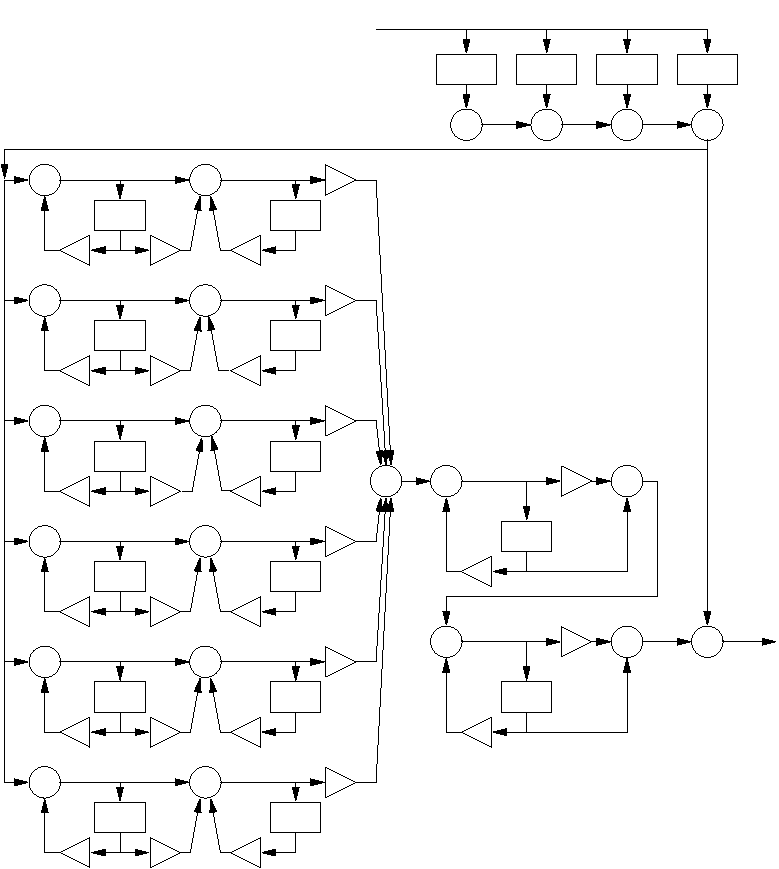
\includegraphics{reverb_serial_des.pdf}%
\end{picture}%
\setlength{\unitlength}{3274sp}%
%
\begingroup\makeatletter\ifx\SetFigFont\undefined%
\gdef\SetFigFont#1#2#3#4#5{%
  \reset@font\fontsize{#1}{#2pt}%
  \fontfamily{#3}\fontseries{#4}\fontshape{#5}%
  \selectfont}%
\fi\endgroup%
\begin{picture}(7317,5055)(-2804,-3178)
\put(-944,434){$b_2$}%
\put(1711,-421){$\Sigma$}%
\put(721,-916){$z^{-d_5}$}%
\put( 91,-421){$\Sigma$}%
\put(1261,-196){-$\alpha_5$}%
\put(2251,-421){$\Sigma$}%
\put(2881,-916){$z^{-d_6}$}%
\put(271,-1006){$\alpha_5$}%
\put(2431,-1006){$\alpha_6$}%
\put(3871,-421){$\Sigma$}%
\put(3421,-196){$-\alpha_6$}%
\put(-449,-421){$\Sigma$}%
\put(-2024,-421){$\alpha_2$}%
\put(-2159,209){$\Sigma$}%
\put(-1529,-286){$z^{-d_2}$}%
\put(-1529,-1546){$z^{-d_3}$}%
\put(-2789,-286){$x[n]$}%
\put(-1529,-2806){$z^{-d_4}$}%
\put(-2159,-2311){$\Sigma$}%
\put(-2024,-2941){$\alpha_4$}%
\put(-944,-2086){$b_4$}%
\put(-2024,-1681){$\alpha_3$}%
\put(-1529,974){$z^{-d_1}$}%
\put(-944,1694){$b_1$}%
\put(-2159,1469){$\Sigma$}%
\put(-2024,839){$a_1$}%
\put(1936,-196){$x_6[n]$}%
\put(4276,-196){$y[n]$}%
\put(-224,-196){$x_5[n]$}%
\put(-1619,1649){$x_1[n]$}%
\put(-1619,389){$x_2[n]$}%
\put(-1619,-871){$x_3[n]$}%
\put(-1619,-2131){$x_4[n]$}%
\put(-2159,-1051){$\Sigma$}%
\put(-944,-826){$b_3$}%
\end{picture}%
  \caption{The figure shows a block diagram of a \gls{reverb} unit.}
  \label{fig:reverb_block_des}
\end{figure}






The equation for the \gls{reverb} can be written in six parts as:


\begin{subequations}
\begin{equation}\label{eq:reverb_eq_1}
w_1[n] = - \alpha \cdot x[n] + x[n-d_1] + \alpha \cdot w_1[n-d_1]
    \end{equation}
\begin{equation}\label{eq:reverb_eq_2}
w_2[n] = - \alpha \cdot w_1[n] + w_1[n-d_2] + \alpha \cdot w_2[n-d_2]
    \end{equation}
\begin{equation}\label{eq:reverb_eq_3}
w_3[n] = - \alpha \cdot w_2[n] + w_2[n-d_3] + \alpha \cdot w_3[n-d_3]
    \end{equation}
    \begin{equation}\label{eq:reverb_eq_4}
w_4[n] = - \alpha \cdot w_3[n] + w_3[n-d_4] + \alpha \cdot w_4[n-d_4]
    \end{equation}
    \begin{equation}\label{eq:reverb_eq_5}
w_5[n] = - \alpha \cdot w_4[n] + w_4[n-d_5] + \alpha \cdot w_5[n-d_5]
    \end{equation}
    \begin{equation}\label{eq:reverb_eq_6}
y[n] = x[n]+w_5[n]
    \end{equation}
 \end{subequations}


\subsection{Matlab Simulation}

A delay can be done in different ways digitally. One way is to use a ring buffer also known as circular buffer. \\
The idea of this data structure is that it takes values and only outputs them when it gets full, and overwrites the oldest after outputting it. It is a kind of a FIFO queue structure but where the start and the overwriting can start at any index. \\
This means that the size of the buffer depends on the delay.  The buffer size must then be always up-to-date with the new delay value. \\ 

The Matlab code for the delay effect is:

\begin{lstlisting}[language=Matlab, caption= Matlab code for delay effect]
clear all
%Delay Effect
%Group 641

%insert your input in this table
filename = 'E_1sec.wav';
[input, fs] = audioread(filename);

%Pre define array and variable
sample_no = length(input); %Length of the input
g = 0.7; %Gain
d = 2000;
x = zeros(1,sample_no+(d*2));
y = zeros(1,sample_no+(d*2));

%Input data to x
for i = 1:1:sample_no-(d+1)
    i = i+d+1;
    x(i) = input(i,2);
end

%Making the delay
for n = 1:1:sample_no %loop for an output with one delay value
    n = n+d+1;   
    y(n) = (-g * x(n)) + (x(n-d)) + (g * y(n-d));
end

%plot
audiowrite('outf.wav',y,fs);
plot(y,'r')
hold on
grid
plot(x,'b')
\end{lstlisting}

